\chapter{Implementation}
The application is implemented as a `mini-app' of the \textit{TrustChain Superapp}~\citep{mattskala2020}. This follows the concept of super apps~\citep{kpmg2019superapps}. The app is published on the Android Play Store\footnote{\url{https://play.google.com/store/apps/details?id=nl.tudelft.trustchain}} and its code is publicly available\footnote{\url{https://github.com/Tim-W/trustchain-superapp}}. As programming language Kotlin is selected, as it is the preferred language for Android development~\citep{googleio2019}. Moreover the underlying technology stack is also written in Kotlin, so this allows for neat integration. This section describes the implementation choices, usage of external libraries and presents the user interface of MusicDAO.

\section{Identity and authenticity}
We implement the public key infrastructure as described in \ref{sec:pki-design}. We use the identity system proposed by \cite{mattskala2020}. All Release blocks (as with all blocks) created on the TrustChain are assigned an identity of the creator. This is a public key using \textit{Curve25519} elliptic-curve cryptography. Every device running the MusicDAO will receive a public/private key-pair upon first launch. While the public key ultimately shows the identification of the device, it can also be used as identification of the artist owning the device. Currently there is no multi-signature support implemented. This means that in the case of a group publishing a Release, there is only one public key representing the whole group. Every artist, and every unique collaboration between artists should generate their own key-pair to describe ownership of the Release.

\section{Metadata storage and discovery}
\subsection{Release blocks}
Releases are objects that represent an audio release produced by one or more artists. This can be an album, an EP, a single, or a podcast. Release objects are stored on the TrustChain, and are exchanged between peers that are part of the MusicCommunity (see \ref{sec:searching-musiccommunity-impl}). These objects are structured as shown in \ref{fig:release-model}. The \textit{magnet} property contains a magnet link which holds all additional information about the contents of the Release, such as the torrent file list, size and tracker URLs. The \textit{publisher} property contains the public key of a Bitcoin wallet which is owned by the creator of the Release. This public key is an identity of the owner of the record (either the artist, band or label). This allows only the owner to receive funds sent by listeners, and no other middlemen (apart from miners).
% When a torrent is created from a local file list, the TorrentInfoName value is established. 

\subsection{MusicCommunity and keyword search}
\label{sec:searching-musiccommunity-impl}
The MusicCommunity extends the TrustChainCommunity with additional methods \textit{performRemoteKeywordSearch} and \textit{onKeywordSearch}. These methods enable searching for content using a keyword, both locally and remotely. These methods test each \textit{title}, \textit{artists} and \textit{date} field of each Release block against a \verb|contain(keyword)| filter. This means: if the keyword is contained in one of those values, it is added to the results.

When the user performs a search, the local database is filtered first to find matches. If there are less than \(x\) results, the device sends a KeywordSearchMessage (see X) to a maximum of \(P\) known peers in the MusicCommunity. This asks neighbours to inspect their local database to find matches for the same query. Upon receival, the peer subtracts 1 from the time to live (TTL) field. If the peer finds a match, it sends the corresponding TrustChain block directly back to the original asker, appointed by the \textit{origin} field. This contains the IPv8 \textit{peer ID}~\citep{mattskala2020} of the peer that initiated the search. Otherwise, if the time to live (TTL) is more than 1, the peer forwards this KeywordSearchMessage (see \ref{fig:keyword-search-message-model}) to other peers. Our keyword search is implemented with default values of \(T=1, P=20, x=5\) (where \(T\) is the TTL).

\section{Networking}
We implement audio track uploading, downloading and streaming using BitTorrent. This technology has shown to run well on mobile devices (cite), allows for extensive configuration and flexible uploading (seeding) strategies. Moreover it supports transfer over local area network and discovering peers in a distributed hash table. It is a well-established technology, as it was released in 2001.

We use the JLibtorrent\footnote{\url{https://github.com/frostwire/frostwire-jlibtorrent}} implementation by Frostwire, which is a Java swig interface for libtorrent\footnote{\url{https://www.libtorrent.org/}}.
\subsection{Torrent creation and sharing}
\label{sec:torrent-creation}
In our application, a user can select local audio tracks, after which a torrent file is generated with the corresponding metadata. Alternatively, the user can paste a preexisting torrent magnet link to use for the Release block, as shown in \ref{fig:select-tracks}. The creation of torrents by the app happens as follows. First, the user presses the \textit{Select Local Audio} button in the release creation dialog (see \ref{fig:submit-release-dialog}). Afterwards, the user selects one or more tracks to add (see \ref{fig:select-tracks}). In the background this creates a torrent file, which is stored on the mobile device and added to the ContentSeeder (see \ref{sec:content-seeding}). Finally, by using the computed infohash and file list, the magnet link of the torrent file is created and added to the \textit{magnet} field of the Release block.

By default, the torrents created using MusicDAO are marked as `trackerless' meaning that torrent peers are found using a distributed hash table~\citep{dht2019} (specifically, mainline DHT\footnote{\url{https://www.libtorrent.org/dht_extensions.html}})instead of centralized trackers. This is to keep the app independent on connectivity on trackers and pushes towards a fully distributed system.

In addition, the app enables the local peer discovery (LPD)~\citep{bittorrentbep142015} functionality of BitTorrent. This allows for finding peers and transmitting torrent pieces over local area network. This results in higher transmission speed and lower latency for content that is stored in the cache of devices nearby. For example, if device A is looking for track X, and device B has this track cached and is active on the same local area network, this track can be found and buffered quickly from A.
\begin{figure}
    \minipage{0.3\textwidth}
        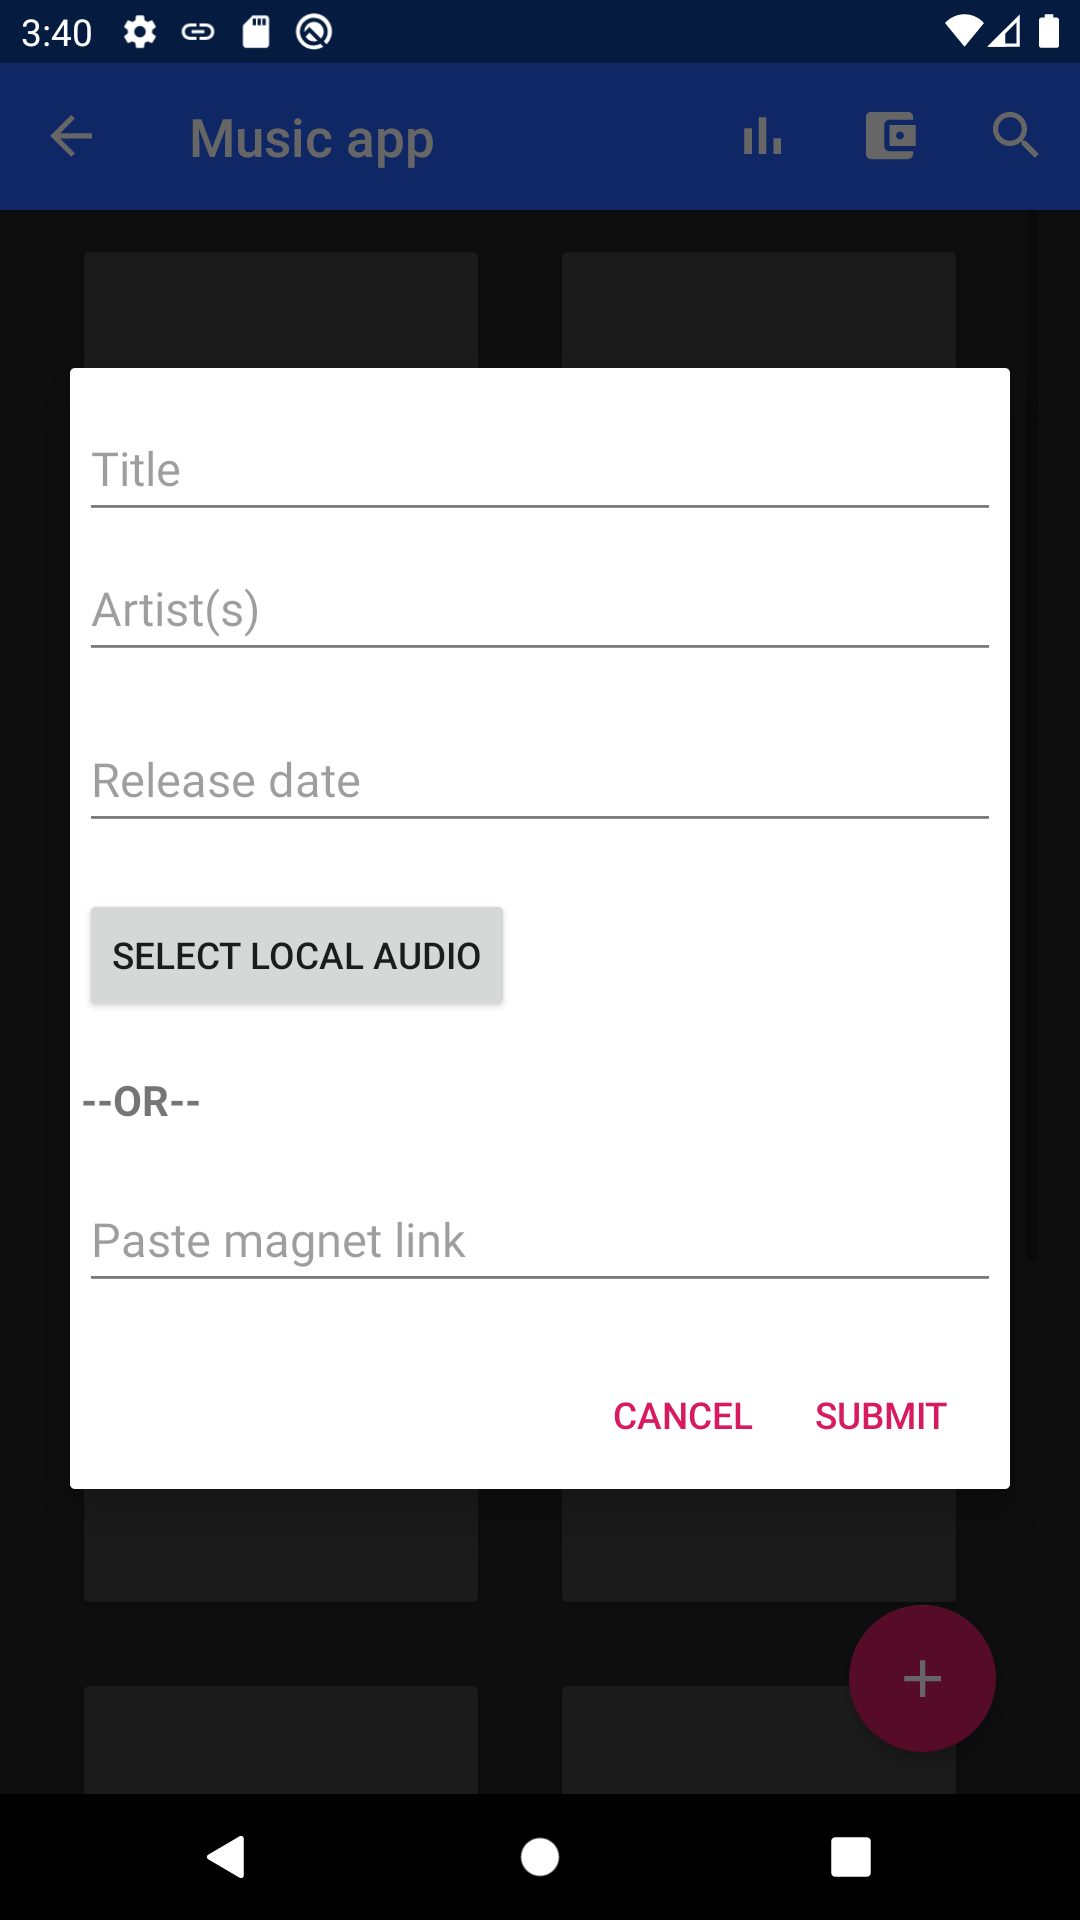
\includegraphics[width=\linewidth]{implementation/screenshot-select-tracks.png}
        \caption{Dialog for creating and publishing a new Release}
        \label{fig:submit-release-dialog}
    \endminipage\hfill
    \minipage{0.3\textwidth}
        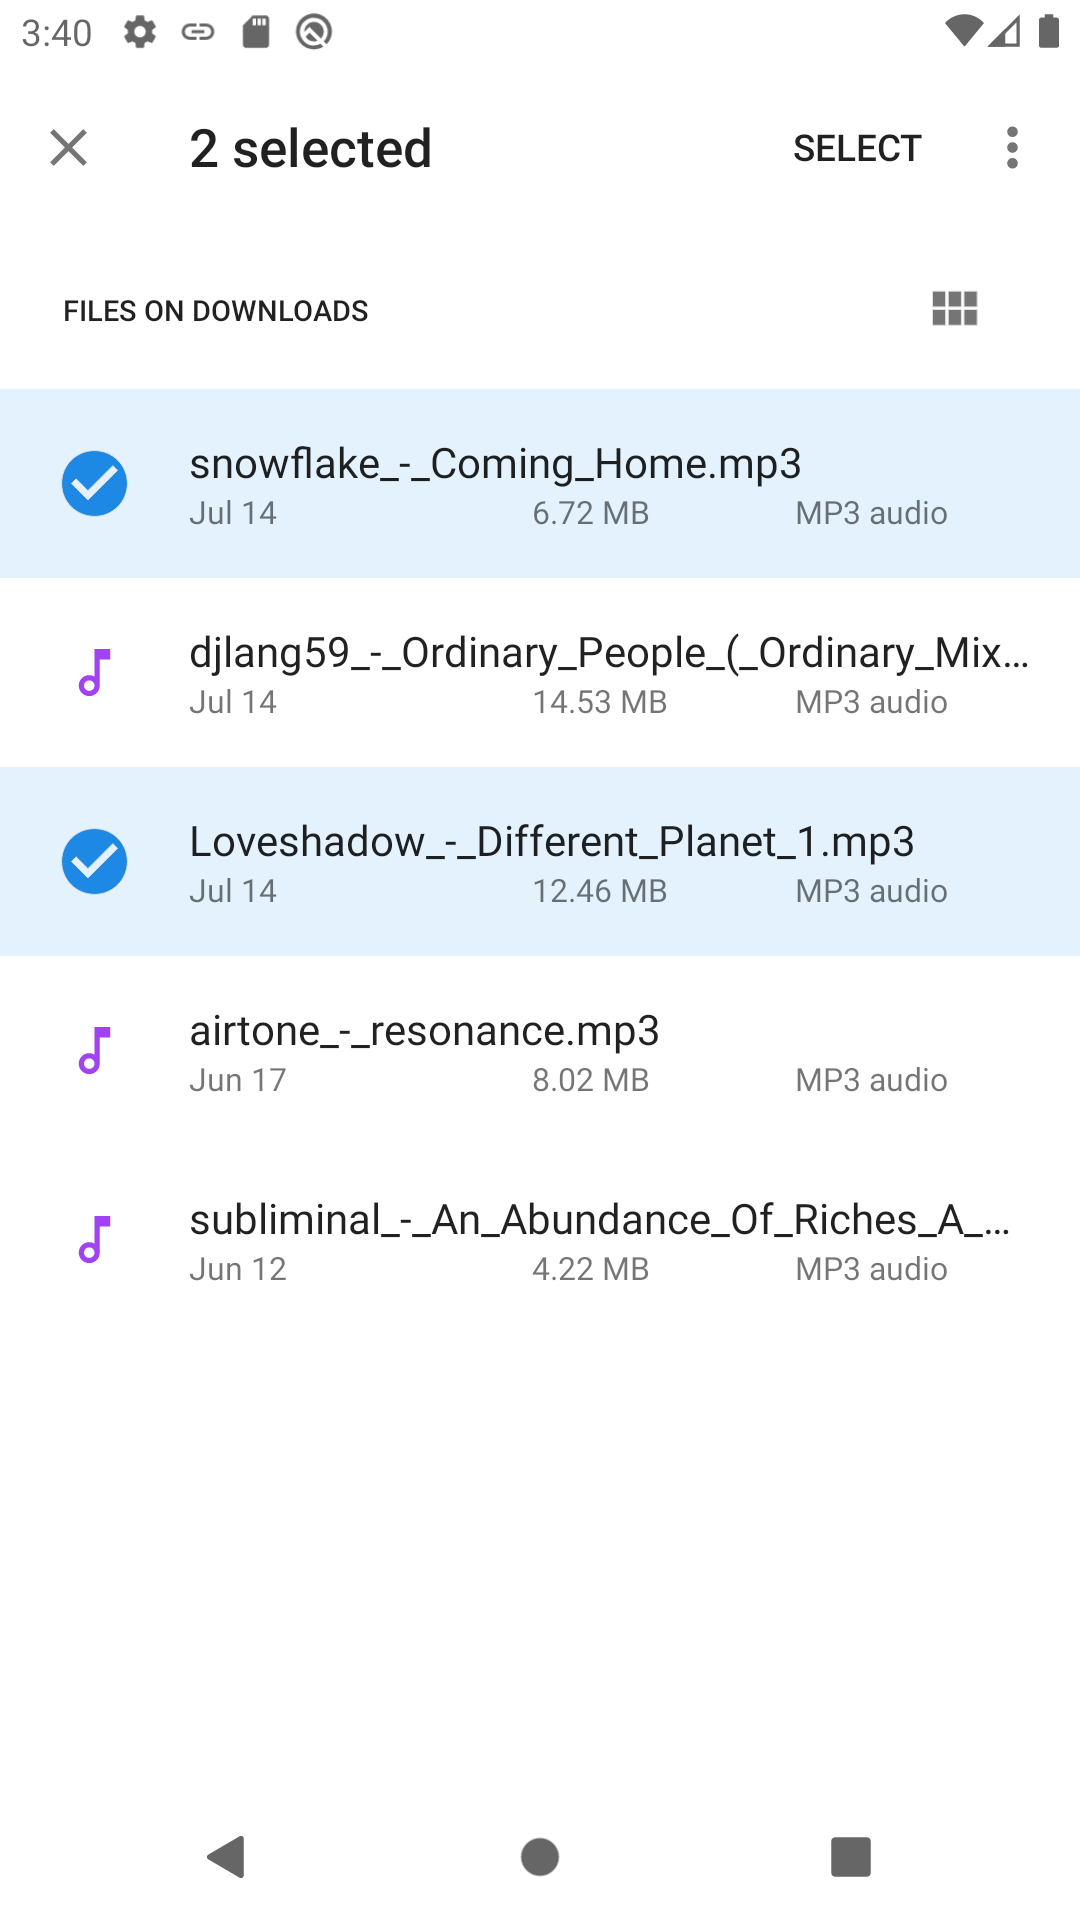
\includegraphics[width=\linewidth]{implementation/screenshot-submit-release.png}
        \caption{Selecting local tracks for creating a new Release}
        \label{fig:select-tracks}
    \endminipage\hfill
    \minipage{0.3\textwidth}
    \endminipage
\end{figure}
\subsection{Content seeding}
\label{sec:content-seeding}
Seeding of content is implemented using a simple continuous mechanism. On startup, the ContentSeeder class (see X) spawns a background thread which iteratively scans all torrent files in the local cache directory of the app. There is an upper threshold for how many torrents are selected for seeding. This threshold \(T\) is currently set to \(T=10\). The ContentSeeder uses a last-in-first-out heuristic: the top \(T\) most recent created/received torrent files are seeded.
\section{Caching}
The app implements both caching of tracks and metadata, to enable fast browsing and playback of tracks. As described in \ref{sec:torrent-creation}, only magnet links are shared on the TrustChain blocks. When the user opens a playlist for the first time, torrent metadata is fetched from peers for the corresponding magnet link. Once this metadata is received, it is written to a new .torrent file in the \textit{cache directory}\footnote{\url{https://developer.android.com/training/data-storage}} of the app. This can then be picked up by the ContentSeeder (see \ref{sec:content-seeding}). The tracks are also stored in the cache directory, in subdirectories identified by the \textit{name}~\citep{bittorrentbep3} property of the torrent metadata. The process of browsing playlists, loading metadata and selecting tracks using caching is shown in fig. \ref{fig:playing-tracks}.
\begin{figure}
    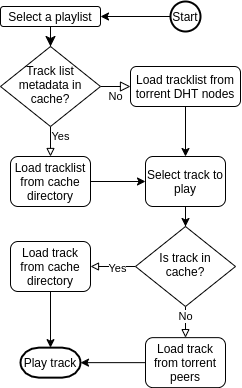
\includegraphics[width=0.3\textwidth]{implementation/playing_track.png}
    \caption{Browsing and playing tracks}
    \label{fig:playing-tracks}
\end{figure}

\section{Music Player and Streaming}
Playing music is implemented using ExoPlayer 2.10\footnote{\url{https://github.com/google/ExoPlayer}}. This music player library is suitable as it allows for playing tracks that are partially loaded, which enables streaming.
\subsection{Priority handling}
To provide the user with selected content as soon as possible, we implemented a system which sets priorities on certain tracks and torrent chunks. This uses the piece priorities system in libtorrent, which range from the integers 1 (normal) to 7 (highest) (see libtorrent Manual\footnote{\url{https://www.libtorrent.org/manual-ref.html\#file-format}}). When a user selects a track, this track is given a \textit{file\_priority} of 5. This is a higher priority than that of other files, so JLibtorrent asks actively for peers who have this file. In addition, the first 5  pieces of the selected track are given a \textit{piece\_priority} of 7, so that the first seconds of the track are buffered quickly and the user can start streaming early.
\subsection{Seeking and buffering}
The music player tries to play the track once a satisfactory portion is loaded. This is implemented as follows. Upon seeking a part of the track, the torrent piece index on which the cursor is located is calculated. Afterwards, the piece at this index and the 5 consequent pieces are given a \textbf{piece\_priority} of 7, which is higher than the other pieces. Once at least 2000 ms from the cursor is buffered, the music player starts playing the track. This way the user can start playing the portion of the track they are most interested in quickly.
\section{Donations and payments}
\subsection{Bitcoin RegTest network}
We created a public Bitcoin RegTest environment\footnote{\url{https://developer.bitcoin.org/examples/testing.html\#regtest-mode}} to test peer-to-peer Bitcoin donations and payments. This creates a new `clean slate' Bitcoin blockchain and allows for full control over the chain and miners. This enables a test environment that is useful for experiments, as we can tweak the block generation speed and keep track of all transactions registered on the closed-off blockchain.
\label{sec:regtest-network-impl}
\section{Interface}
\subsection{Playlist overview}
The playlist overview screen, as shown in \ref{fig:screenshot-home} is the screen that is first shown upon starting the MusicDAO. Here the user is presented a list of playlists, loaded from their local TrustChain database. Currently, each Playlist fragment corresponds to exactly one Release block (see ref). In the background runs an iterative process which checks whether new playlist content is found, and re-renders the view if necessary. The playlists are sorted on their torrent swarm health in ascending order. 
\begin{figure}
    \minipage{0.3\textwidth}
        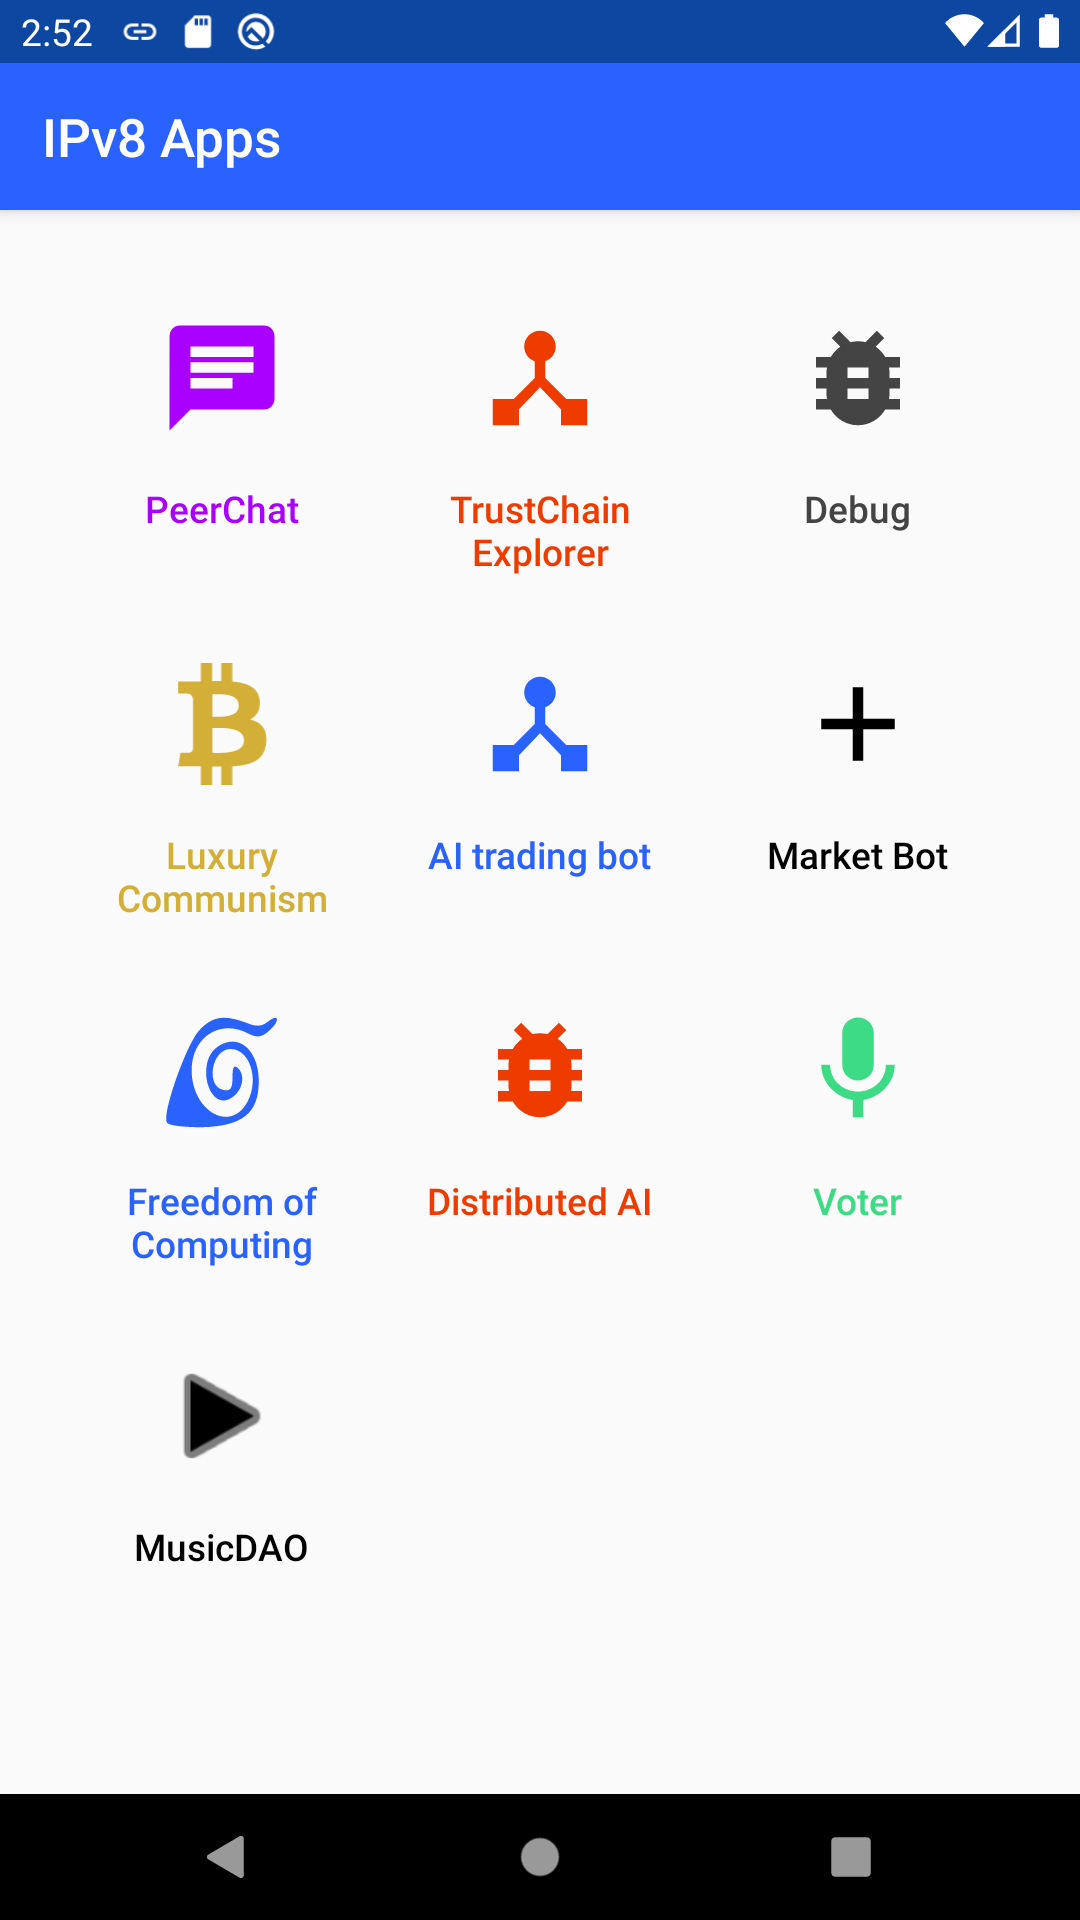
\includegraphics[width=1\linewidth]{implementation/screenshot-superapp.png}
        \caption{The app is integrated as a mini-app in the IPv8 Superapp catalog}
        \label{fig:screenshot-superapp}
    \endminipage\hfill
    \minipage{0.3\textwidth}
        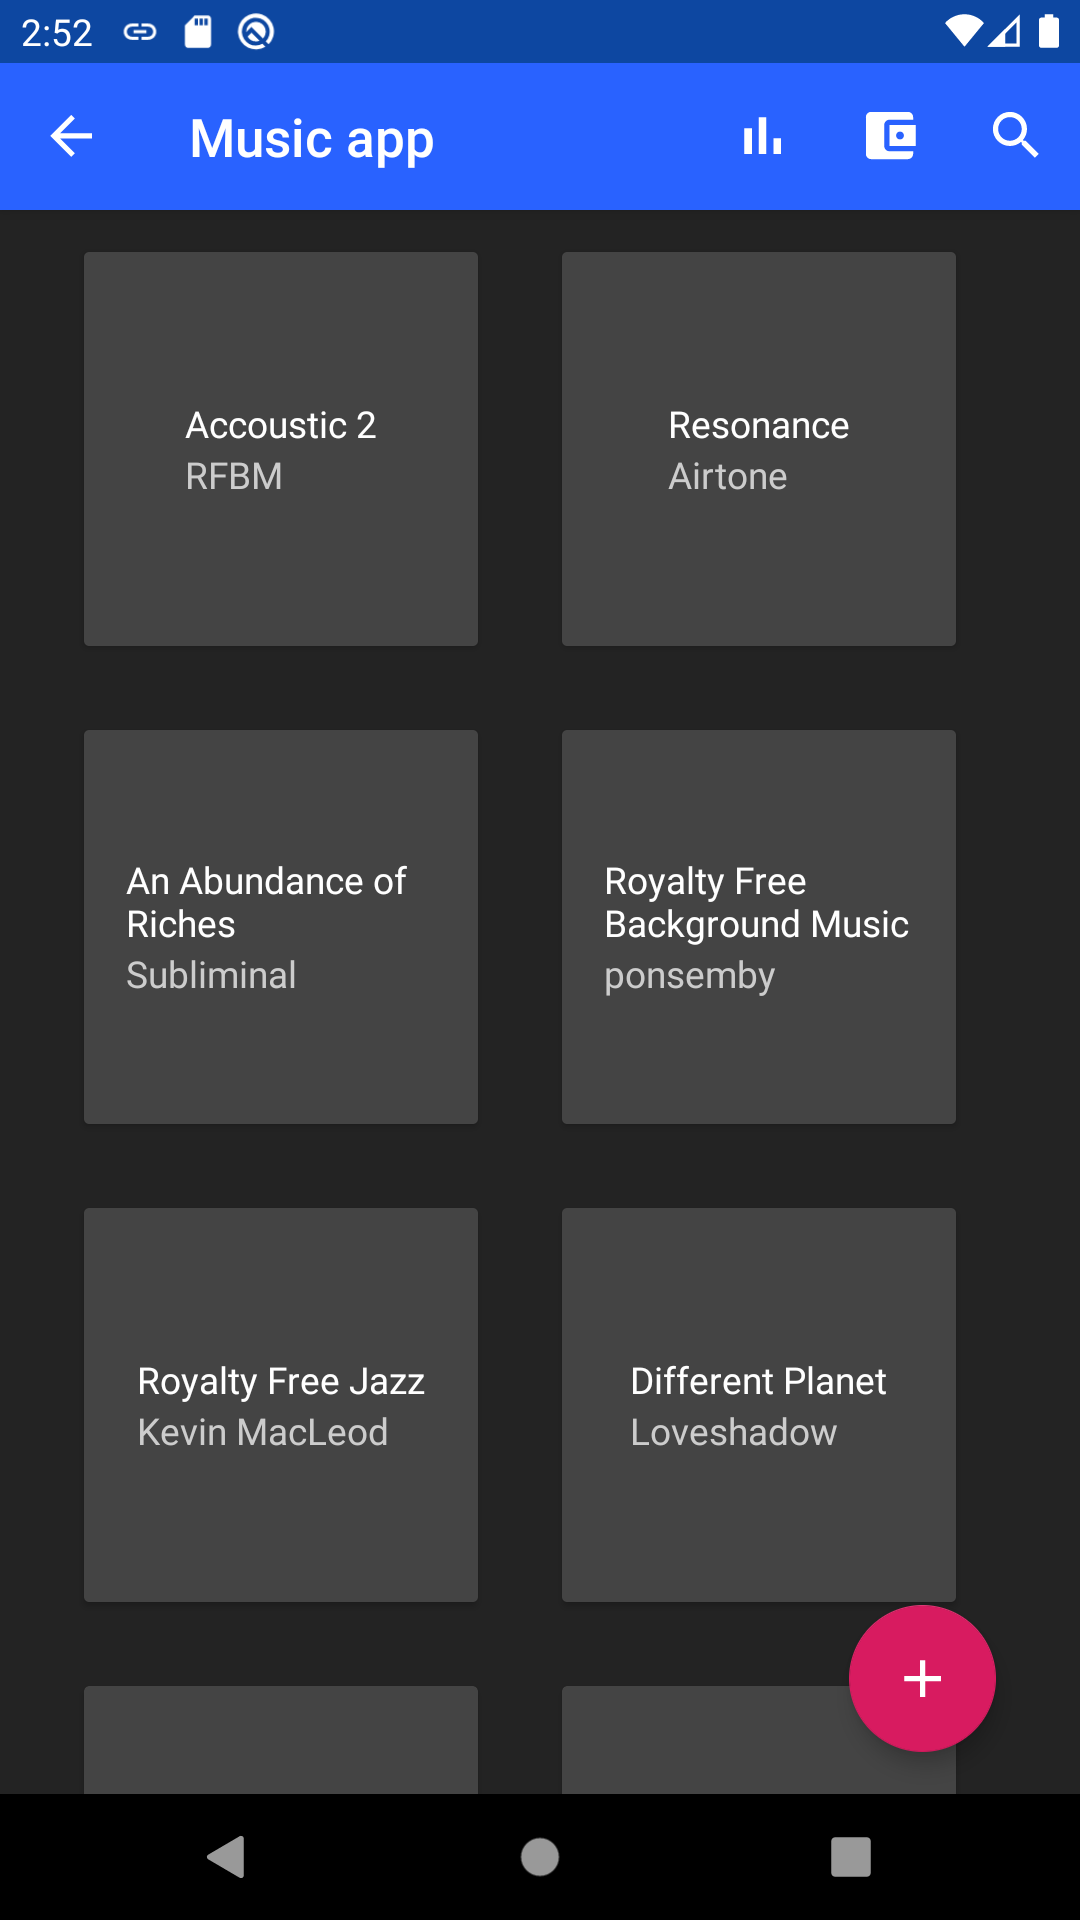
\includegraphics[width=1\linewidth]{implementation/screenshot-home.png}
        \caption{The playlist overview screen, which is the entrance screen}
        \label{fig:screenshot-home}
    \endminipage\hfill
    \minipage{0.3\textwidth}
        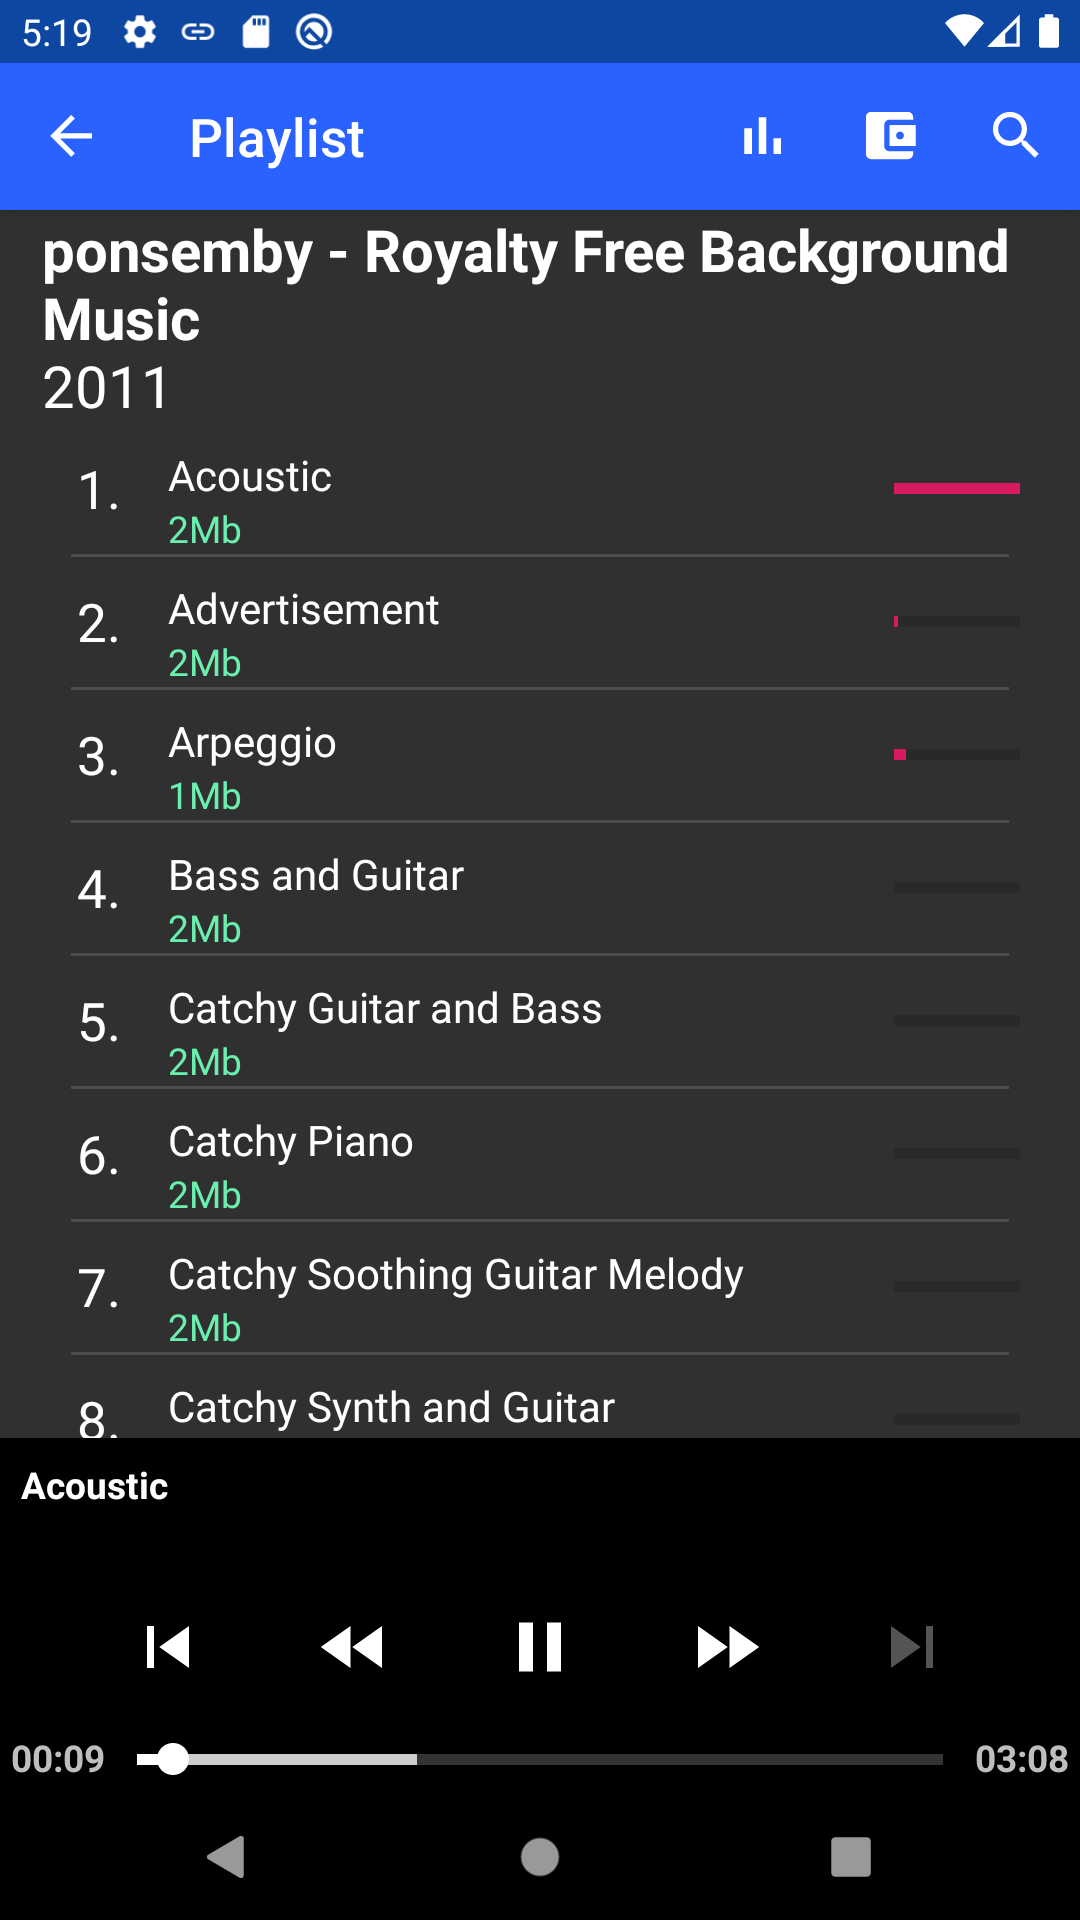
\includegraphics[width=1\linewidth]{implementation/screenshot-playlist.png}
        \caption{Playlist fragment, showing all tracks of one Release}
        \label{fig:screenshot-playlist}
    \endminipage\hfill
\end{figure}
\subsection{Playlist fragment}
A Playlist fragment displays one Release object. The playlist fragment shows its list of tracks and other metadata, such as the title and artists of the Release (see \ref{fig:screenshot-playlist}). For each track the file size is displayed, and a loading indicator on the right side. This shows, in real time, how much of the track is downloaded. In the example of \ref{fig:screenshot-playlist}, the first track is fully loaded.
\subsection{Wallet}
Each device participating in the MusicCommunity is given a private/public wallet identity upon installation of the MusicDAO. The wallet interface (fig. \ref{fig:wallet-sync}) shows synchronization status of the RegTest network (see \ref{sec:regtest-network-impl}). Once the wallet is fully synchronized with the blockchain, the private key and balance are displayed as shown in fig. \ref{fig:wallet-balance}. 

Upon browsing a playlist, if the \textit{publisher} field is present in the corresponding Release object, a donation button is displayed as shown in fig. \ref{fig:tip-artist}. When pressing this button, the user can select an amount and make a direct donation to the artist or band, in the form of a bitcoin transaction from their wallet. The user enters a value in USD and the corresponding amount in bitcoin is calculated and shown when this field is edited. This is implemented using the XChange library\footnote{\url{https://github.com/knowm/XChange/releases/tag/xchange-5.0.1}} connecting to the Binance trading platform\footnote{\url{https://www.binance.com/en/trade/BTC_USDT}}. After confirmation, the transaction is registered on the RegTest network (see \ref{sec:regtest-network-impl}). 
\begin{figure}
    \minipage{0.3\textwidth}
        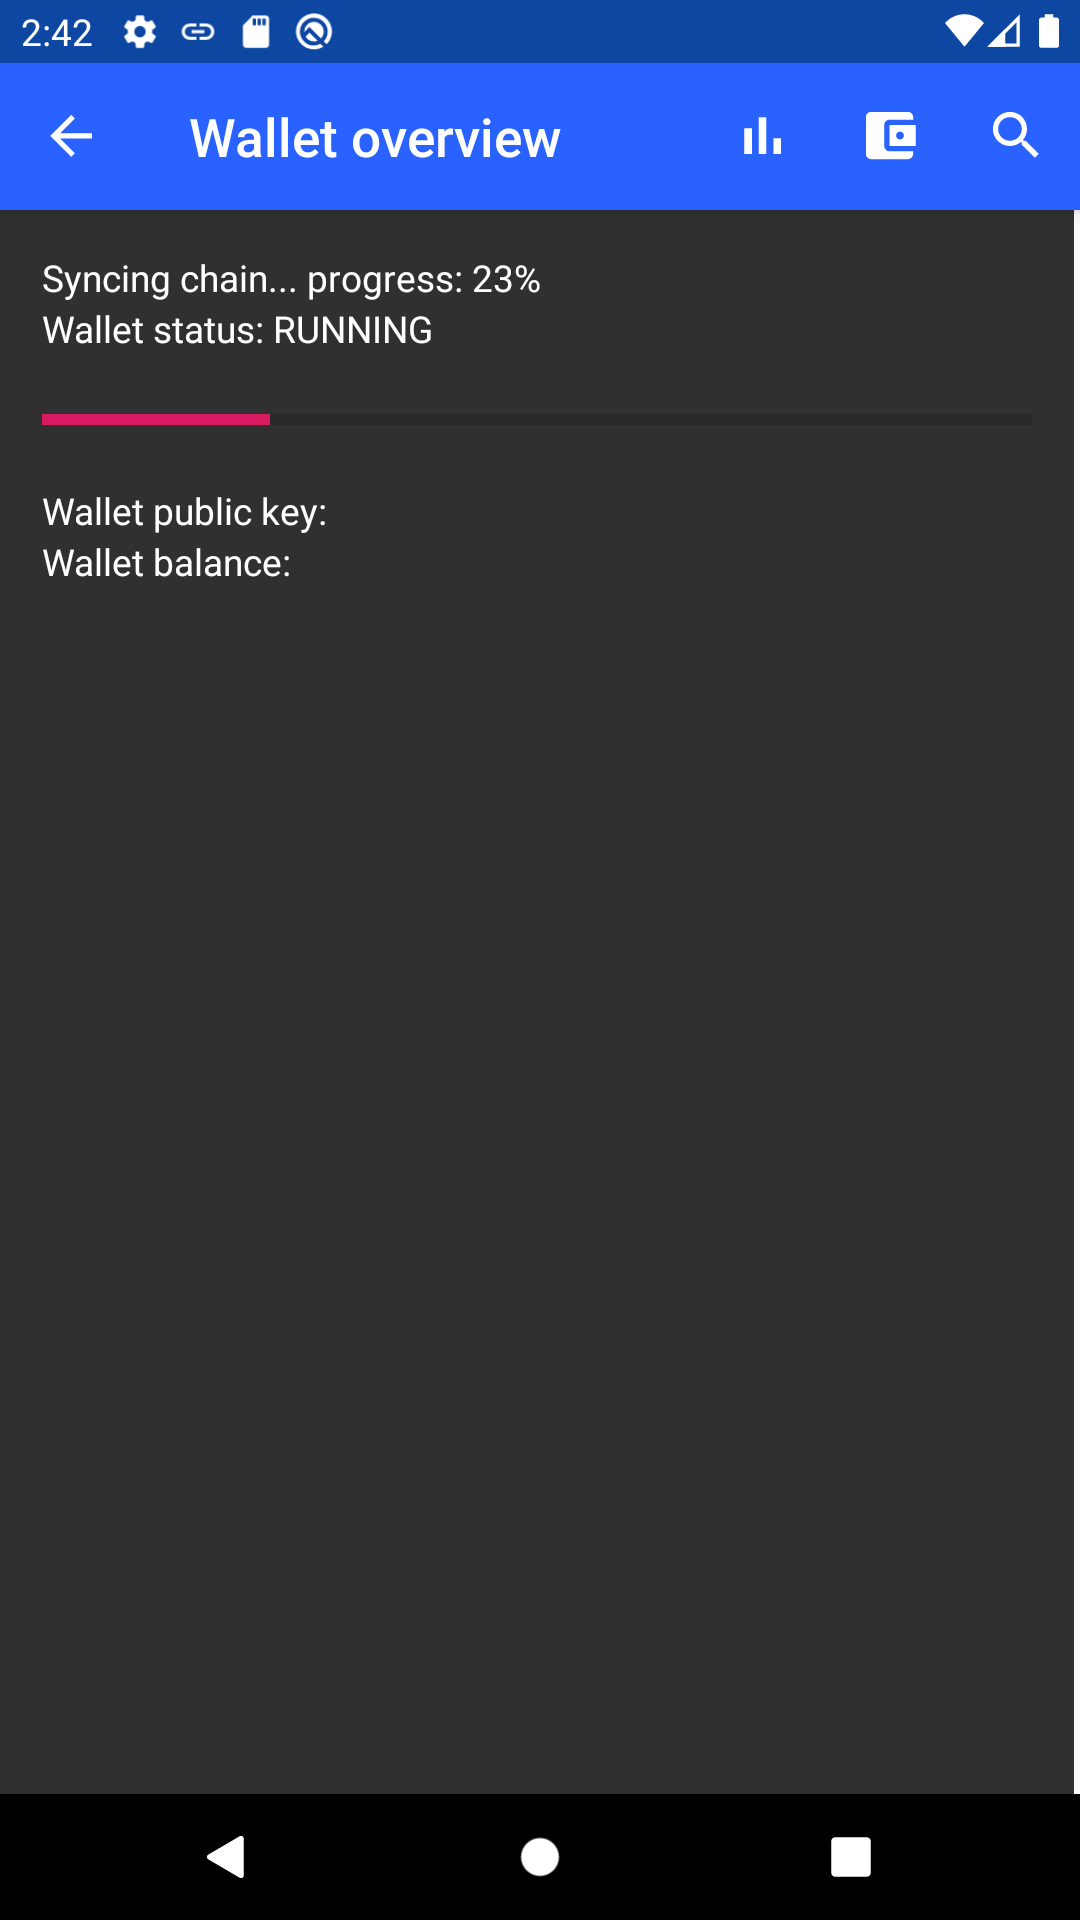
\includegraphics[width=1\linewidth]{implementation/wallet-sync.png}
        \caption{Synchronizing with the Bitcoin RegTest environment blockchain}
        \label{fig:wallet-sync}
    \endminipage\hfill
    \minipage{0.3\textwidth}
        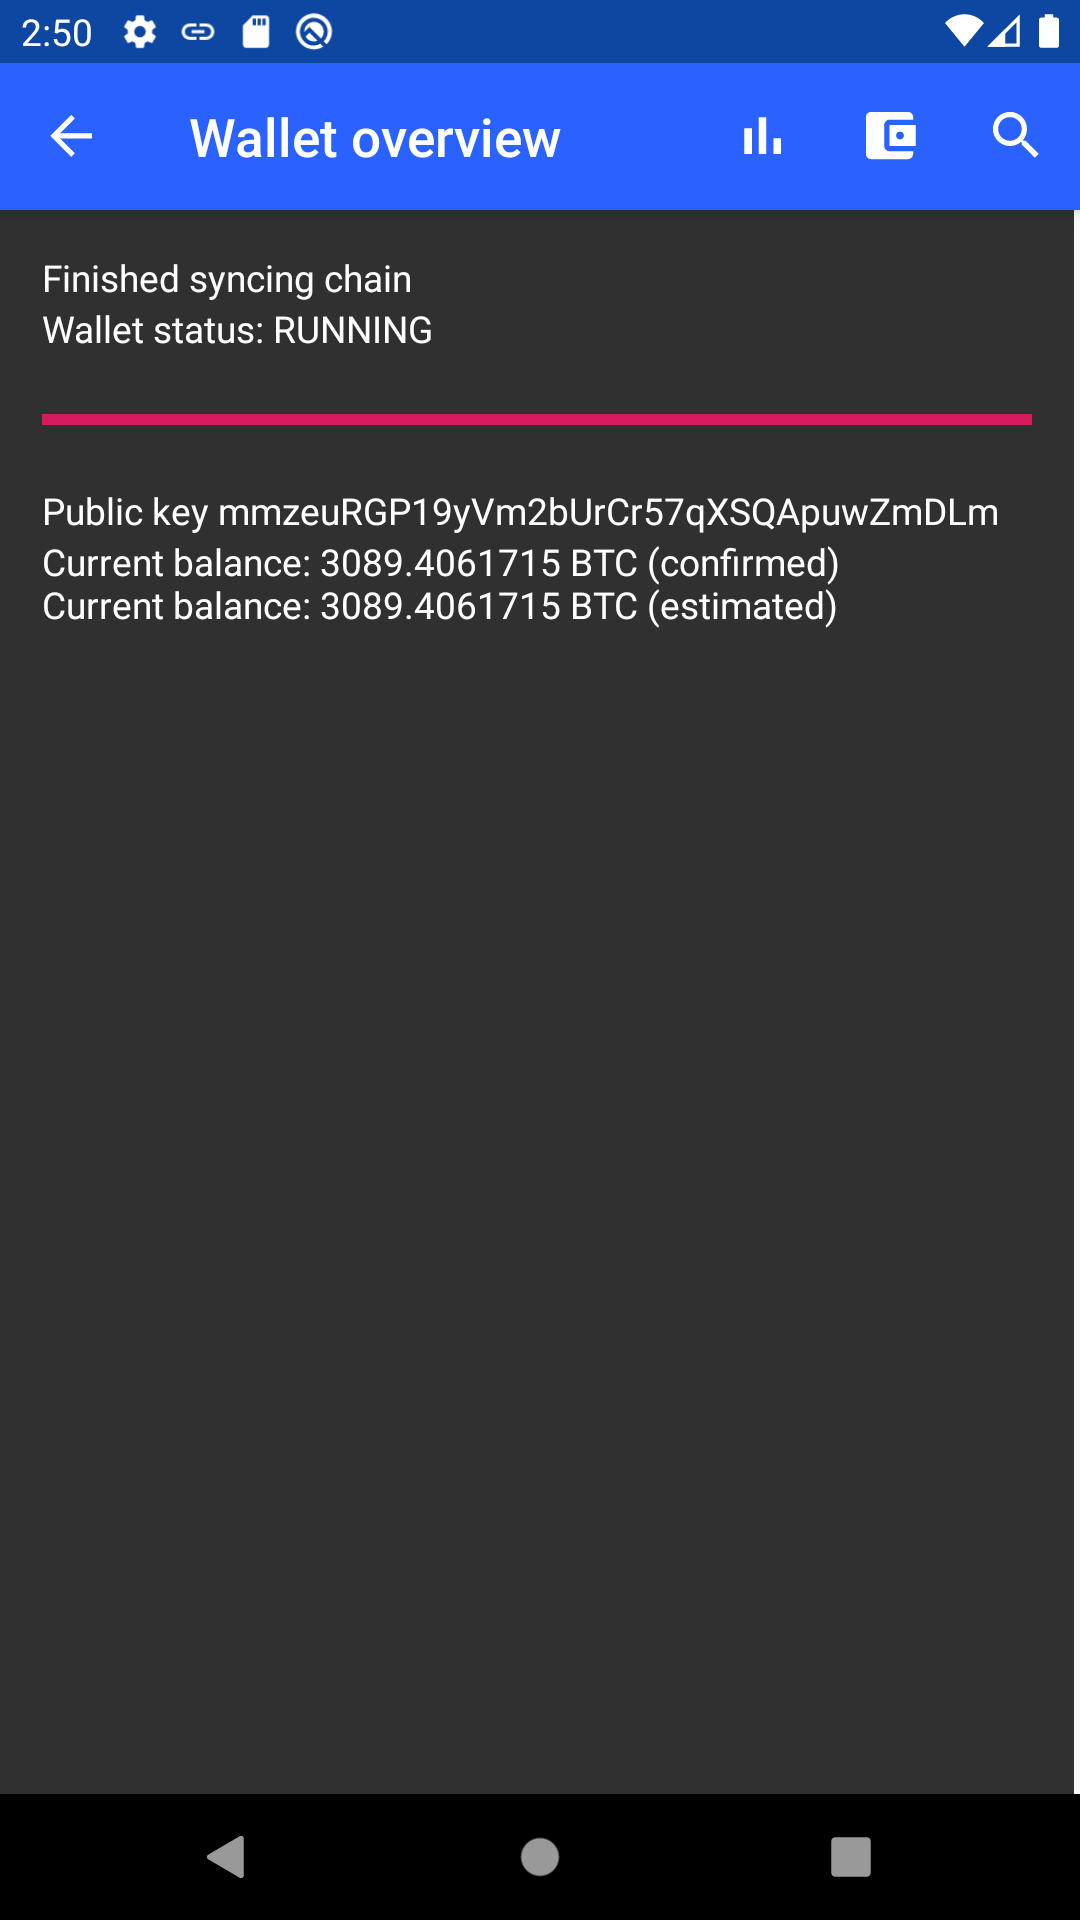
\includegraphics[width=1\linewidth]{implementation/wallet-balance.png}
        \caption{Wallet overview and balance after synchronizing}
        \label{fig:wallet-balance}
    \endminipage\hfill
    \minipage{0.3\textwidth}
        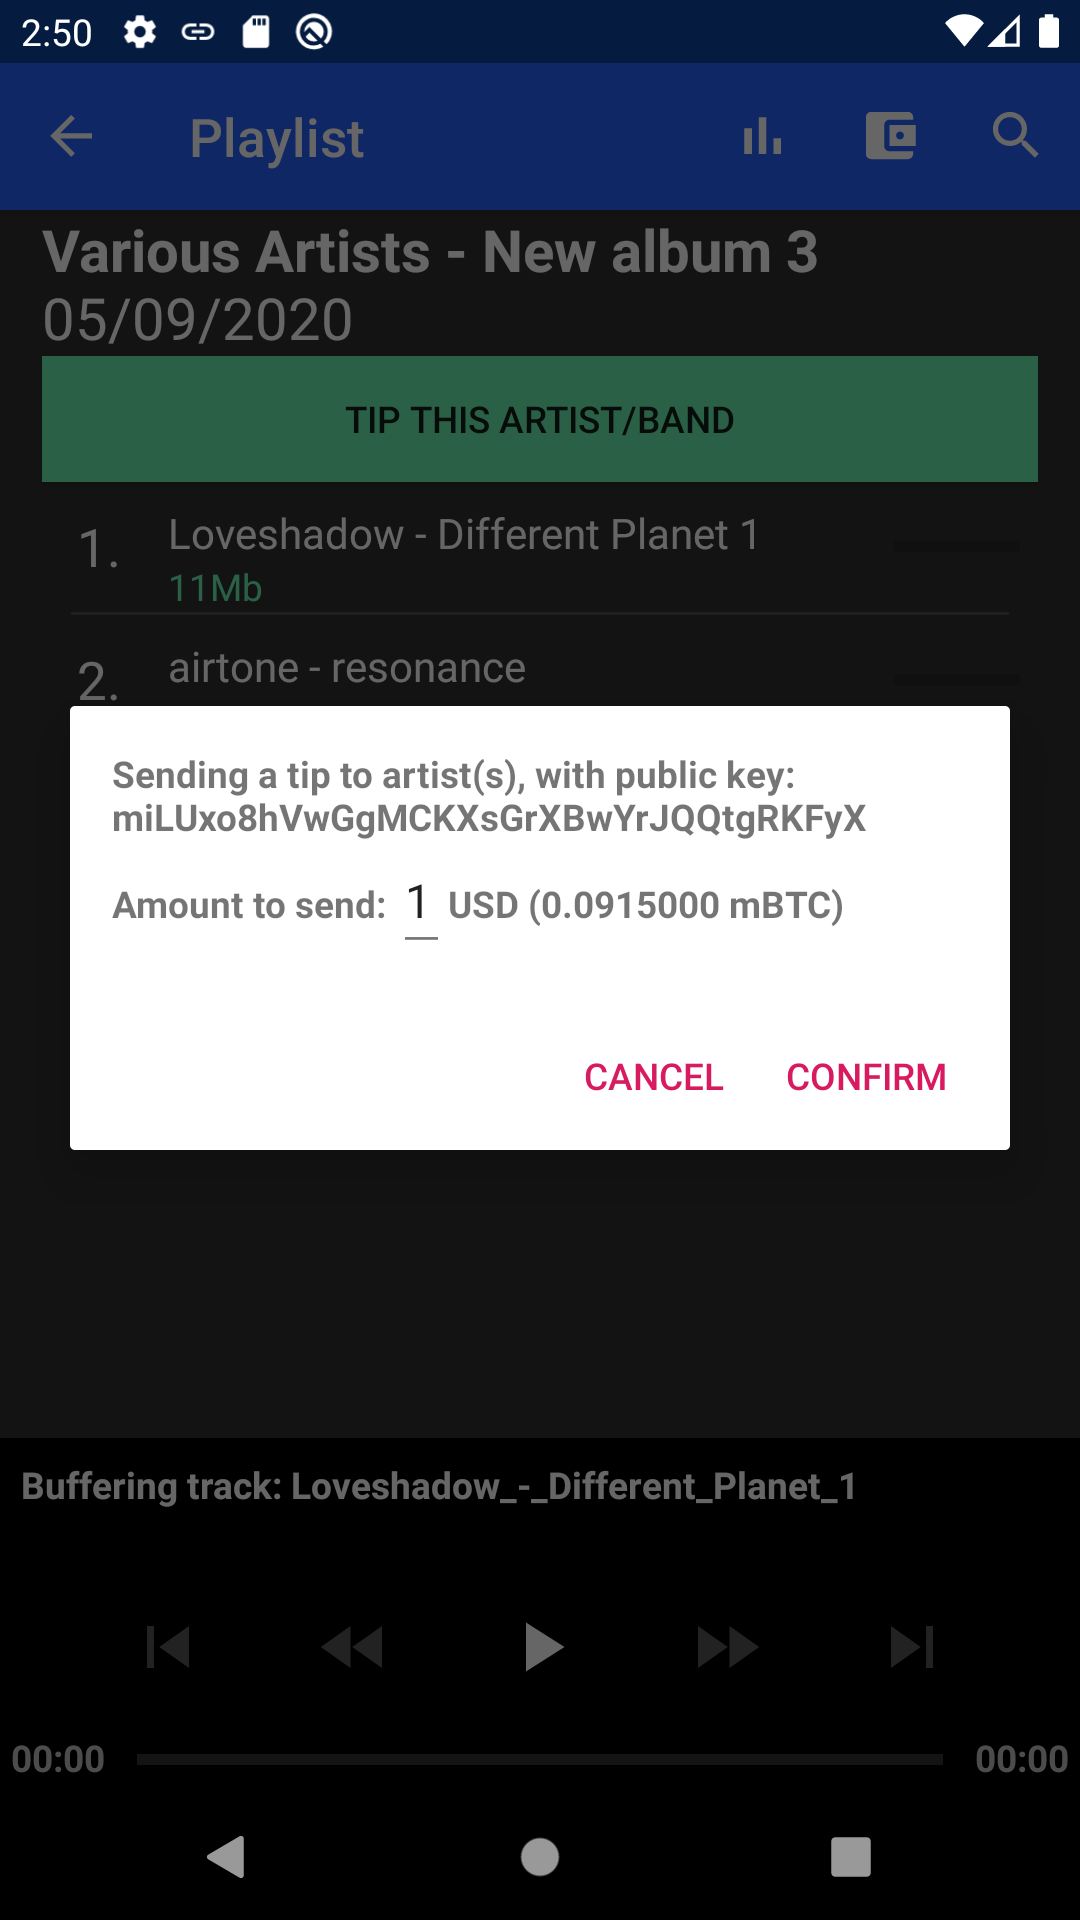
\includegraphics[width=1\linewidth]{implementation/tip-artist.png}
        \caption{Sending a tip to an artist or band}
        \label{fig:tip-artist}
    \endminipage\hfill
\end{figure}